
\documentclass[11pt, doublespacing]{article}  
\usepackage{epsfig}
\usepackage{subfigure}
\usepackage{url}
\usepackage{graphicx}

%\usepackage{wrapfigure}
\usepackage{setspace} 
\usepackage{amsmath}
\usepackage{amssymb}
%\renewcommand{\familydefault}{\sfdefault}
%\usepackage[tight,footnotesize]{subfigure}

%\newtheorem{Rule}{Rule}
\def\httilde{\mbox{\tt\raisebox{-.5ex}{\symbol{126}}}}

\setlength{\oddsidemargin}{0in}  
\setlength{\textwidth}{6.5in}  
\setlength{\textheight}{8.8in}  
\setlength{\topmargin}{0in}  
\setlength{\headheight}{0in}  
\setlength{\headsep}{0in} 

\begin{document}


\section*{RI: Small: Deep Learning in Forensic Impression Evidence Comparison}
\vspace{0.5in}
\section{INTRODUCTION}

This research will address a need of the forensic sciences using recent developments in machine learning. The forensic sciences have been under great stress in recent years with a  decline in public and judicial confidence  in the abilities of scientists in the courtroom \cite{NAS09, Daeid2015}. A case in point is the analysis of impression evidence, e.g., footwear prints, latent prints, handwriting, tire treads, etc. 
A  human expert, i.e., a forensic scientist,  performs side-by-side comparison of the evidence with a known, e.g., a questioned signature with known signatures, a crime scene shoe-print with suspect footwear, a latent fingerprint found in a crime scene with a database of  fingerprints, etc, and expresses a conclusion as one of three discrete statements: individualization, no opinion and exclusion. In  several court cases  the final  judgment of guilty/innocent has been subsequently found to be in error, e.g., by a later assessment using DNA analysis.   

The need to characterize uncertainty of the conclusion in the form of a likelihood ratio (LR)  is now recognized as being essential to reporting forensic comparison results \cite{Neumann2007,Srihari2008,Taylor12}. LR is defined as the ratio of the joint probability of evidence and known under two alternative hypotheses(same/different). The LR can be subsequently used with appropriate priors to determine the posterior probability. In the case of handwriting, each of the evidence and known are represented by  a set of features by a Forensic Document Examiner (FDE)-- the features being chosen for  distinguishing between writers  \cite{Muehlberger1977}.   Features for comparing handwritten {\em th} are shown in Fig. \ref{fig:th-features}. 

The result of comparing the known feature vector ${\mathbf{\phi}_k}$ and the evidence feature vector ${\mathbf \phi}_e$ is expressed as an LR.  
The numerator of the LR, which corresponds to  the same source hypothesis $h^0$,  is the joint probability of  ${\mathbf \phi}_e$ and ${\mathbf{\phi}_k}$ when both arise from the same individual. The denominator, which corresponds to the different source hypothesis $h^1$, is the  joint probability of the evidence and known when they arise from different individuals. Thus we can write
\begin{equation}
 LR(\phi_{k},\phi_{e})=\frac{p[({\bf \phi}_k,{\bf \phi}_e) | h^{0}]}{p[({\bf \phi}_k ,{\bf \phi}_e) | h^{1}]}.
\label{eq:LRJ}
\end{equation} 
where the numerator and denominator are  two distributions, the first conditioned on being  from the {\em same} source  and the second from  {\em different} sources.
The LR can be used in a Bayesian formulation to provide posterior odds-- which is computed as the product of prior odds and LR , i.e., 
\begin{equation}
O_{posterior}(k:e)=LR(\phi_{k},\phi_{e}) \times O_{prior}(k:e)
\label{eq:Odds}
\end{equation}
 The prior odds  can be obtained from the population of suspects, e.g., if there are $n$ equally likely suspects then $p(h^{0})=1/n$, then $p(h^{1})=(n-1)/n$ and $O_{prior} \approx 1/n$.  Fig. \ref{fig:LR} shows the prior and posterior odds for $LR=10^6$ for different  $n$ \cite{Taylor12}. 

\begin{figure}
\label{fig:th}
\centering
%\begin{minipage}{.2\linewidth}
\subfigure[First Writer]
{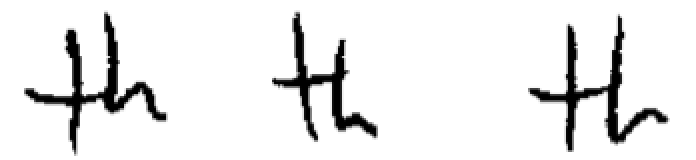
\includegraphics[width=0.4\linewidth]{Figures/th1}}\hfill
\subfigure[Second Writer]
{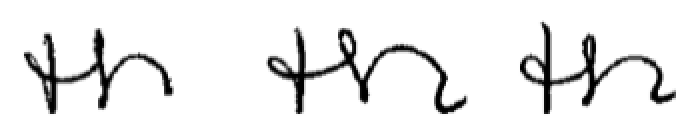
\includegraphics[width=0.4\linewidth]{Figures/th2}}
%\end{minipage}
\caption{\small Handwriting of two individuals (three samples). One set of features extracted per writer. } 
\end{figure}

\begin{figure}

\subfigure[$\phi = {[} Val(R),Val(L),Val(A),Val(C),Val(B),Val(S) {]}$.]
{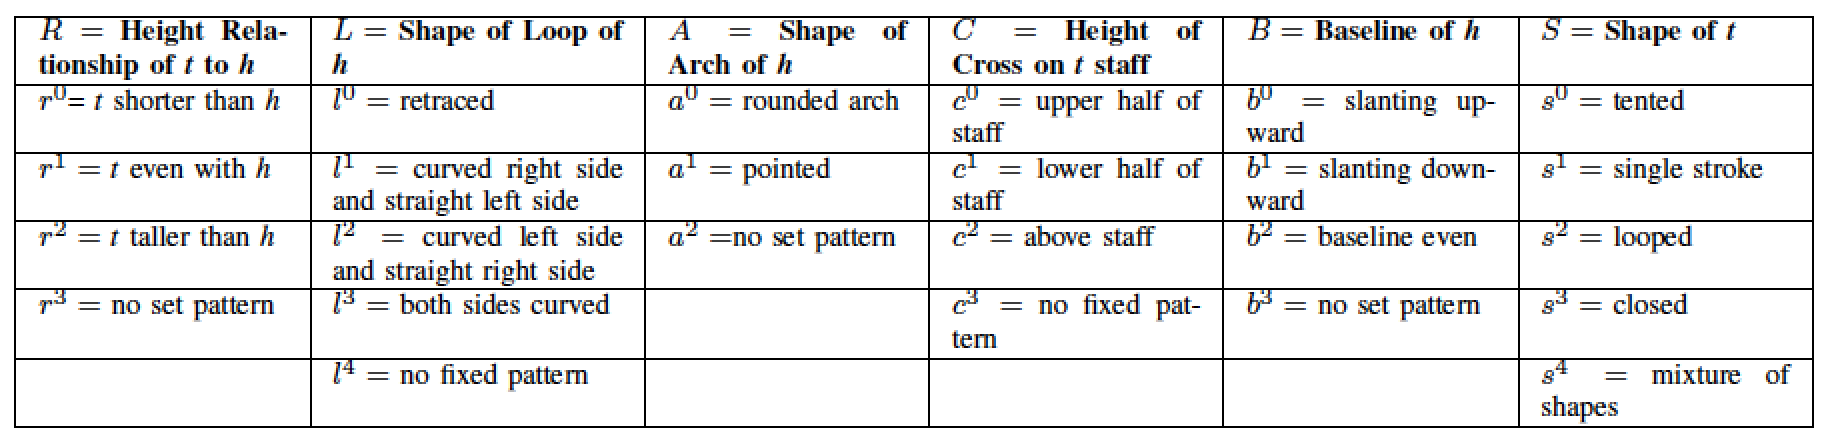
\includegraphics[width=0.78\linewidth]{Figures/th-features}}
\subfigure[Bayesian network ]
{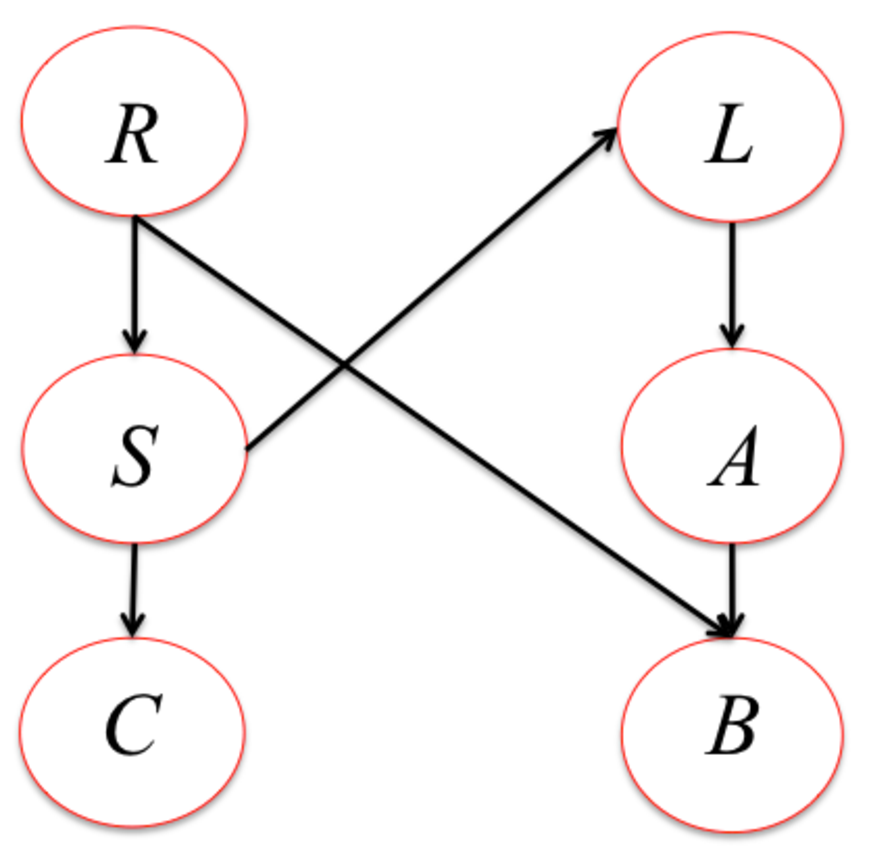
\includegraphics[width=0.2\linewidth]{Figures/BN-th}}
\caption{\small{Expert features for {\em th}: (a) values, and (b) a Bayesian network $BN_{th}$ for its probability distribution. The full distribution needs $ 4,799$ joint probabilities while $BN_{th}$ needs only $100$ conditional probabilities \cite{srihari2011}.}}
\label{fig:th-features}
\end{figure}



\begin{figure}

\centering
%\begin{minipage}{0.6\linewidth}
\centering
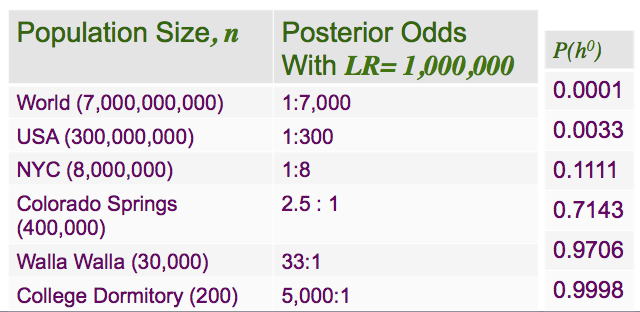
\includegraphics[width=0.3\linewidth]{Figures/Priors-posteriors}
%\end{minipage}
%\begin{minipage}{0.35\linewidth}
%\centering
\caption{\small{Different populations of size $n$ and corresponding posterior odds when likelihood ratio is $10^6$ (From \cite{Taylor12}). The last column shows the posterior odds converted to the probability of $h^0$.}}
%\end{minipage}
\label{fig:LR}
\end{figure}

Evaluating LR by directly computing (\ref{eq:LRJ}) is intractable since it requires two joint probabilities in high-dimensional feature space, e.g., for {\em th} shown in Figure \ref{fig:th-features} each distribution would have 36 variables requiring 23 million probabilities, and even a Bayesian network that captures conditional independences \cite{Koller2009} would be quite complex. One simplification is to use distributions of a kernel function $d(\phi_{k},\phi_{e})$ leading to a definition $LR_D$ as follows:
\begin{equation}
 LR_{D}(\phi_{k},\phi_{e})=\frac{p[d({\bf \phi}_{k},{\bf \phi}_{e}) |h^{0}]} 
{p[d({\bf \phi}_{k} ,{\bf \phi}_{e}) |h^{1}]}.
\label{eq:LRD}
\end{equation} 
This method is used in some handwriting and speaker verification systems \cite{Srihari2007}. While it straightforward to evaluate (\ref{eq:LRD}), it is a severe approximation of (\ref{eq:LRJ}) since it  effectively projects a multidimensional distribution into a single dimension. A compromise is an approximation that factorizes the LR  into similarity and rarity terms,  $LR_{DR}$ \cite{Lindley1977,Tang-Srihari14} defined as:
\begin{equation}
 LR_{DR}(\phi_{k},\phi_{e})={p[d({\bf \phi}_k,{\bf \phi}_e)|h^{0}]} \times \frac 1{p[{\frac 12} ({\bf \phi}_k + {\bf \phi}_{e})] }.
\label{eq:LRF}
\end{equation} 
The factorization in (\ref{eq:LRF}) is intuitively appealing since a human expert gives more importance to unusual features, i.e.,  low probability  (rare) features are given higher weight \cite{Su2010}. This method of LR computation is interestingly analogous to TF-IDF used in information retrieval. However the computational complexity is similar to (\ref{eq:LRJ}).


\begin{figure}
\centering
%\begin{minipage}{0.4\linewidth}
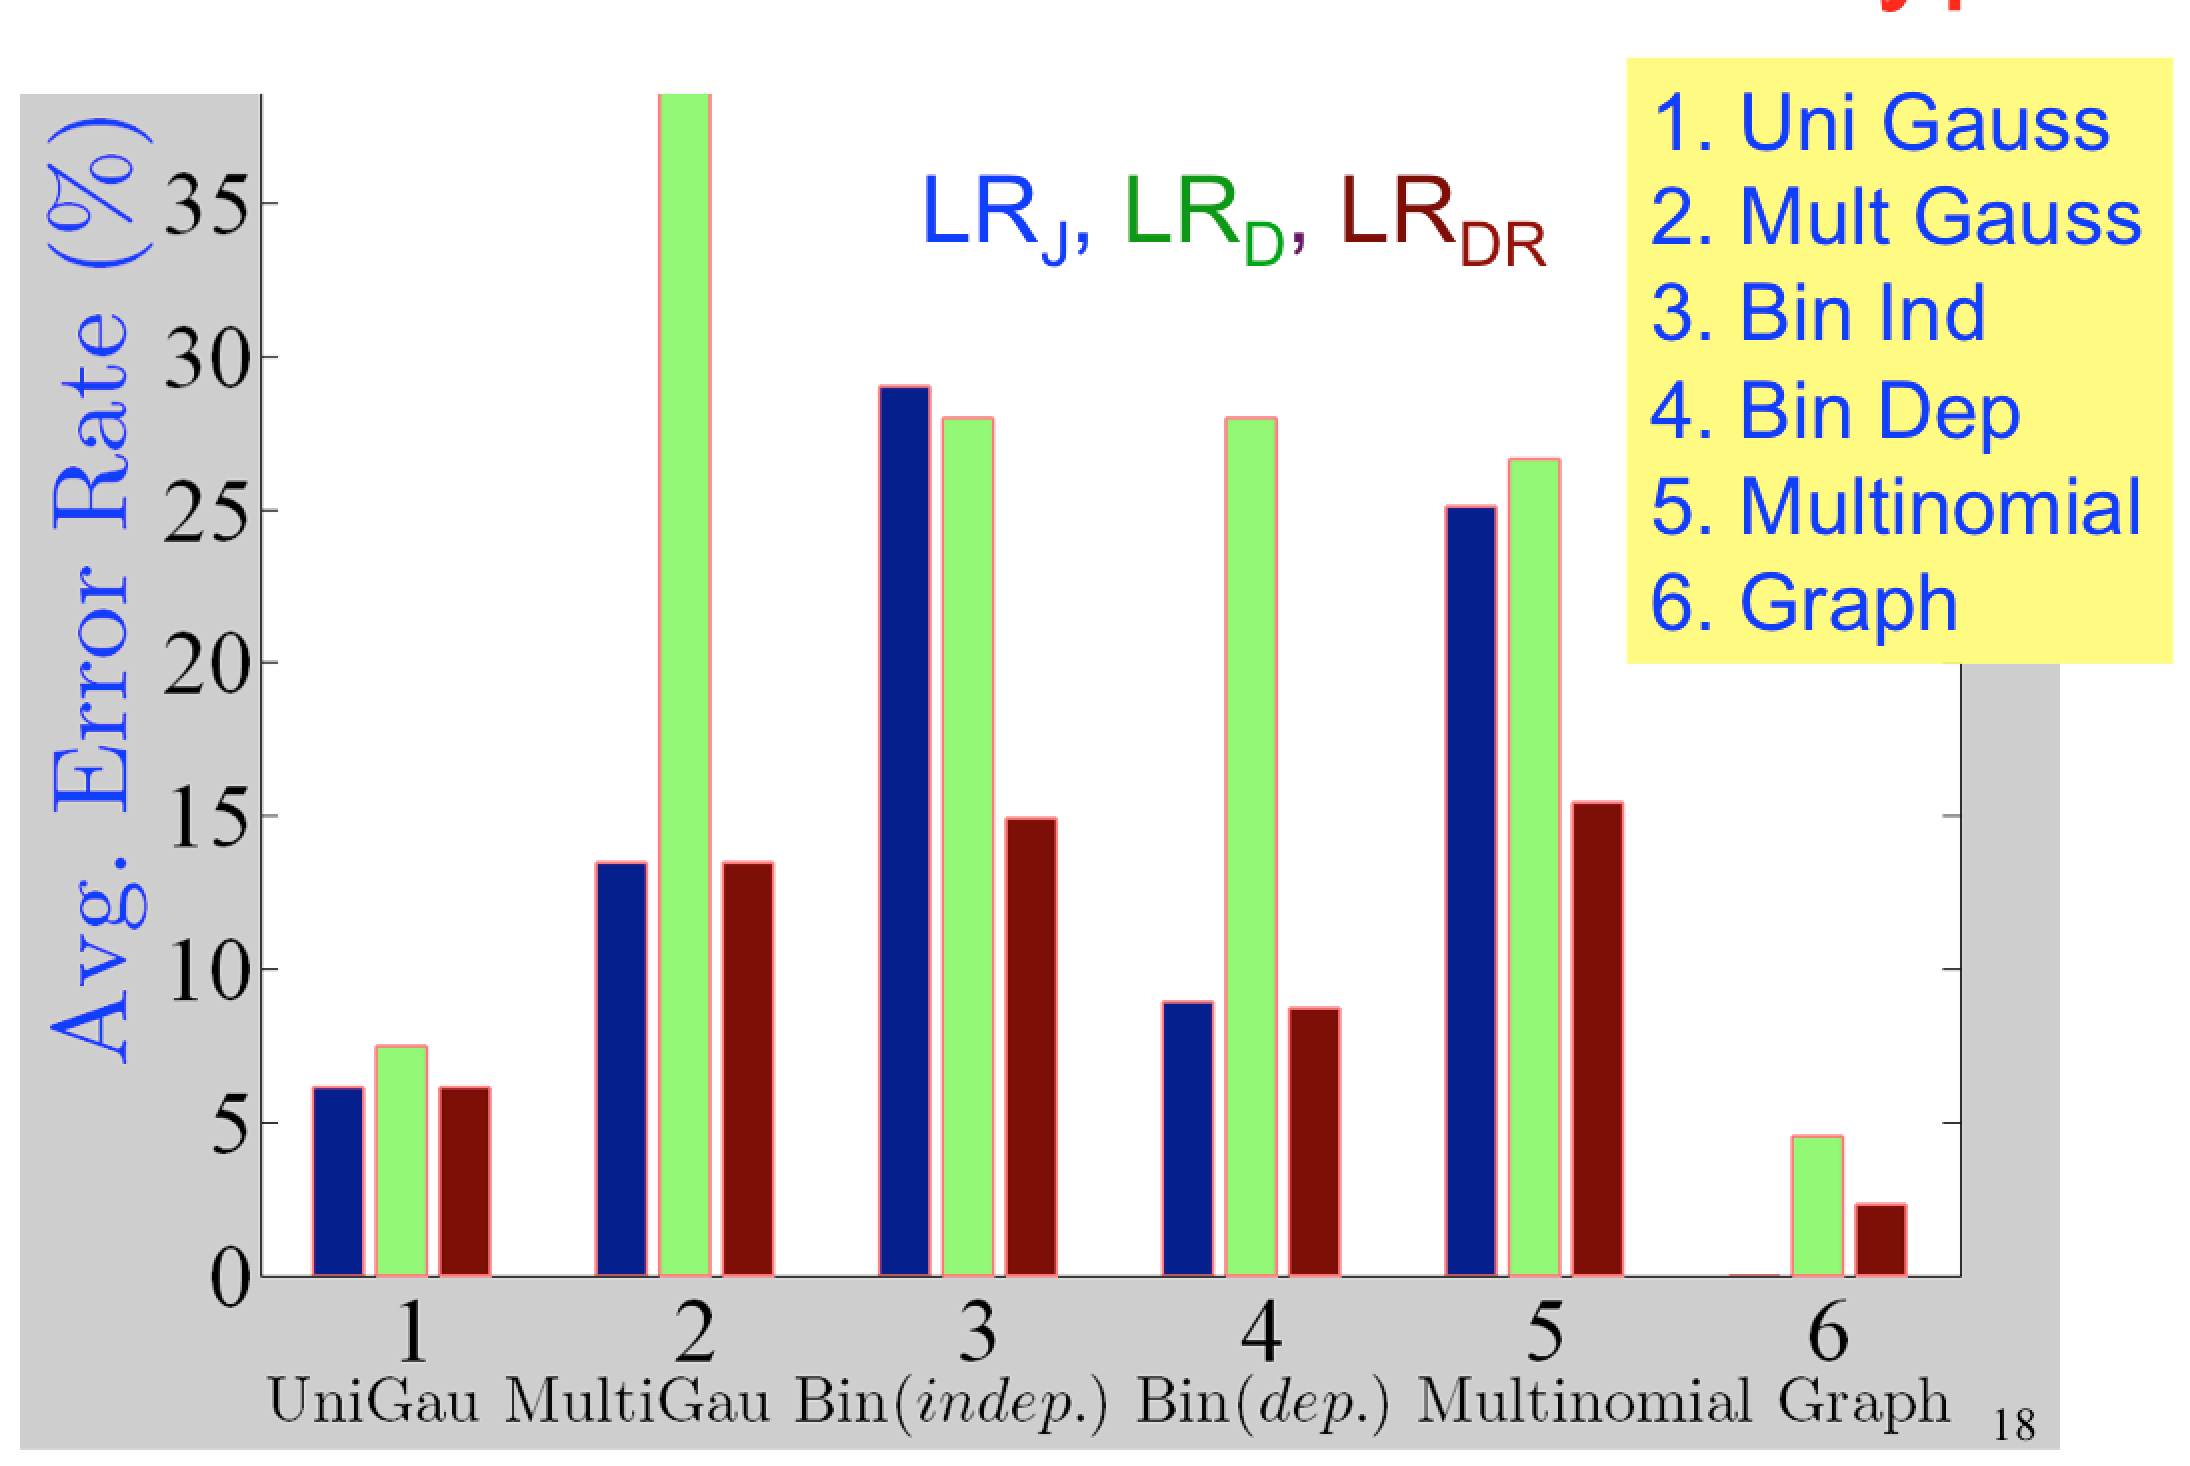
\includegraphics [width=0.3\linewidth]{Figures/LRperformance}
%\end{minipage}
%\begin{minipage}{0.45\linewidth}
%\centering
\caption{\small{Average error rates of three generative approaches to determine likelihood ratiio:  $LR$(blue), $LR_{D}$(green) and $LR_{DR}$(red). Six data sets were used: univariate Gaussian, multivariate Gaussian, independent binary features, correlated binary features, multinomial distributions and graphs. Overall, $LR_D$ has the highest error and  $LR_{DR}$  has the lowest error. The $LR$ method was approximated with independence assumptions, and hence is not the best \cite{Tang-Srihari14}.}}
%\end{minipage}
\label{fig:LRperformance}
\end{figure}

Thus we have three methods of LR computation: (i)  direct evaluation using (\ref{eq:LRJ}), (ii) kernel evaluation using (\ref{eq:LRD}), and (iii) factorization using (\ref{eq:LRF}).
A comparison of the performance of the three methods is shown in Fig. \ref{fig:LRperformance} \cite{Tang-Srihari14}. Each of the three methods  have two serious practical limitations, both of which we propose to address in this research. 
\begin{enumerate}
\item {\em Intractability:} All three are {\em generative}  probabilistic models which  require a full representation of the necessary probability distributions \cite{Bishop2006}. It is prohibitively expensive to construct for (\ref{eq:LRJ}), e.g., even  for the six variable discrete distribution  shown in Fig. \ref{fig:th-features},  we would need 12 variables to represent both $\phi _k$ and $\phi _ e$ which in turn would need 23 million probabilities for each of the two hypotheses. In general, if we have $n$ features taking $k$ values each, we would need $2k^{2n}$ probabilities, which is exponential in complexity. Even a Bayesian network of $2n$ variables would require a huge numbers of samples.
\item {\em Human Engineering:} All three rely on  hand-crafted features $\phi$ designed by human experts  such as in Fig. \ref{fig:th-features}(a). It is impractical to define different sets of features for comparisons of different handwritten words, footwear types, etc. Features hand-crafted for each application is subject to bias-- which is of significant concern to the judicial system.
\end{enumerate}

In this research we propose to  overcome  intractability  by using a {\em discriminative} approach. Instead of separately learning the two probability distributions in (\ref{eq:LRJ}), we would train them jointly.  A discriminative model would express LR as:
\begin{equation}
LR(\phi_{k},\phi_{e})=f(\phi_{k}, \phi_{e}, {\boldmath {\mathrm w}})
\end{equation}
where $\boldmath {\mathrm w}$ is a set of parameters. A neural network would determine the parameters as those  that maximize the likelihood of a set of training samples, or equivalently minimize the cross-entropy error
\footnote{ Likelihood and cross-entropy error are defined as follows. Denoting  $\phi_=(\phi_{k},\phi_{e})$, and given data set $(\phi_{n},t_{n}), n=1,..,N$ of labeled known-evidence pairs,  the likelihood is $p({\boldmath \mathrm {t|w}})=\prod_{n=1}^{N}y_{n}^{t_{n}}(1-y_{n})^{1-t_{n}}$, where ${\boldmath \mathrm t}=[t_{1},..,t_{N}]^t$ and for a no-hidden layer neural network (logistic regression)  $y_{n}=\sigma ({\boldmath \mathrm w}^{t}\phi_{n})$. Cross-entropy error is $E({\boldmath \mathrm w})=-\ln p({\boldmath \mathrm {t|w}} )=-\sum_{n=1}^{N}  \left[ t_{n}\ln y_{n}+(1-t_{n})\ln(1-y_{n})\right]$. Since there is no closed-form solution for minimizing $E({\boldmath \mathrm w})$, gradient descent of the form ${\boldmath {\mathrm w}}^{\tau +1}={\boldmath {\mathrm w}}^{\tau }-\eta \nabla E$ is used. The partial derivatives $\nabla E$  are determined by error backpropagation, whose complexity is $O(W^{2})$, where $W$ is the total number of adaptive parameters.}.
The function $f$ for a single hidden layer neural network is given in (\ref{eq:discriminative}) and (\ref{eq:neuralnet}).

Eliminating human engineered features is possible with {\em deep learning}, a machine learning approach that has shown spectacular results in many tasks such as object recognition,  speech recognition, computer vision, natural language processing, etc. 
The principal advantage of deep learning is that the necessary representation is automatically learnt in a supervised manner.  
However the architecture for forensic comparison needs to be fundamentally different.  Object recognition typically works with a single image as input and object classes are widely different, e.g., cat versus dog, different people, handwritten digits, etc. Whereas forensic comparison takes a pair of inputs as input with both having many major features in common, e.g., {\em th} written by two people.

An important extension of the model described is to compute the cumulative LR over several comparisons, e.,g., comparison of multiple handwritten words/notes or  several footwear impressions in a crime scene.  An example is shown in Fig. \ref{fig:US-examples} where  phrases, rather than words,  are compared.  While methods of fusing multiple classifiers \cite{Ho1994} are relevant, explicit methods of combining LRs may be more useful \cite{Kovalenko2012}. Recurrent neural networks are also a possible solution \cite{LeCun2015}.
\begin{figure}[htb]
\centering
\subfigure[Writer 1]
{
\includegraphics[width=0.45\linewidth]{Figures/USExample1}}\hfill
\subfigure[Writer 2]
{
\includegraphics[width=0.45\linewidth]{Figures/USExample2}}
\caption{\small Comparison of  phrase of words ($K=8$) written by two individuals: need to combine  eight LRs.} 
\label{fig:US-examples}
\end{figure}



\section{OTHER PREVIOUS WORK IN FORENSIC COMPARISON}
\label{PreviousWork}
\subsection{Generative Models}
With the relatively  recent realization that forensic opinion needs to be accompanied with a characterization of uncertainty, several researchers have proposed LR methods. However the methods proposed are all based on  either (i) modeling probability distributions of features or (ii) modeling distributions of similarity measures for computing  $LR_D$ \cite{Neumann2007,Taylor12}.
A generative method of computing $LR_D$  using  (\ref{eq:LRD})  with  eleven feature differences together with a naiive Bayes model, is used in the CEDAR-FOX software system \cite{Srihari2007}. The  software further maps the  $LR_D$  to a discrete  opinion scale based on their distribution \cite{Srihari2008a}. The nine-point FDE scale has the opinions: {\em identified-as-same, highly-probable-same, probably-did, indications-did, no-opinion, indications-did-not, probably-did-not, highly-probable-did-not, identified as elimination} \cite{Srihari2014a}.

\subsection{Discriminative Models}
Although neural network training  using stochastic gradient descent (SGD)  has been around for several decades \cite{Bishop2006},  the forensic sciences have not benefited.  
As an experimental system, a single hidden layer network was used to compare handwriting samples in \cite{Srihari2002} (Fig. \ref{fig:NN-JFS})-- to determine same/different writer. Input consisted of eleven differences (distances) corresponding to eleven features.  This architecture is a  discriminative method for computing  $LR_D$, see (\ref{eq:LRD}), rather than $LR$. 
\begin{figure}
\centering
%\begin{minipage}{0.7\linewidth}
%\centering
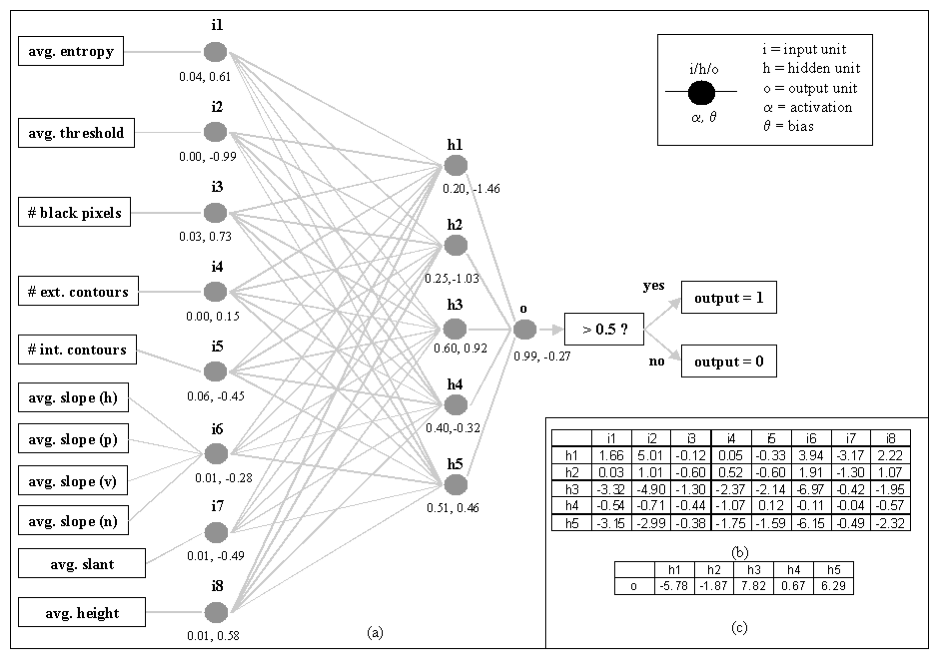
\includegraphics[width=0.5\linewidth]{Figures/NeuralNetworkJFS}
%\end{minipage}
%\begin{minipage}{0.25\linewidth}
%\centering
\caption{\small{A neural network for  handwriting comparison using feature dissimilarity. Input consists of differences of eleven features. There are five hidden units and  a single output unit \cite{Srihari2002}.}}
%\end{minipage}
\label{fig:NN-JFS}
\end{figure}

The proposed research will move away from computing $LR_{D}$ (used in both \cite{Srihari2002} and  \cite{Srihari2007}) and compute the full $LR$ based on a complete representation of $\phi_{k} $ and $\phi_{e}$. This will take us into a much higher level of complexity than hitherto attempted in any forensics sub-discipline.
The effort   is encouraged by the success of deep learning \cite{LeCun2015}, where the system learns representations with multiple levels of abstraction. Deep learning has dramatically improved the state of the art in speech recognition, visual object recognition \cite{Krizhevsky2012}, object detection, drug discovery and genomics. They dispense with careful engineering and domain expertise needed to transform raw data into a feature vector.  In particular convolutional networks, where earlier layers alternate between convolutional and pooling layers,  which are trained jointly using  backward error propagation and SGD, have demonstrated invariance to pose, lighting, background, and surrounding objects. Another approach is to determine high-level features using large-scale unsupervised learning using Restricted Boltzmann Machines (RBM) in a generative way \cite{Le2012}.


\subsection{Footwear impression comparison}
This problem is a difficult one that has very little automation: at best a human identifies features interactively, which are then used  to query a database of footwear outsoles. Our previous effort in developing an algorithm for comparing  footwear impressions  is shown in Figure \ref{fig:Footwear}. In this method,  a distance (or similarity) between evidence and known is computed. The distance is based on using computer vision techniques to extract features (centers of circles and ellipses).  A relational graph is constructed from these points. Finally a distance between graphs is computed.  Thus at best we can determine $LR_D$  rather than $LR$ by using this method.  A comprehensive survey and comparison of automated methods for footwear impression comparison can be found in our report \cite{Srihari2011a,Srihari2014}.
\begin{figure}
\centering
%\begin{minipage}{.6\linewidth}
%\centering
\subfigure[Evidence]{
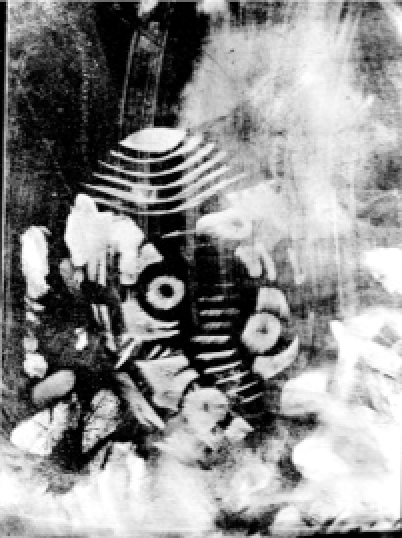
\includegraphics [width= 0.1\linewidth]{Figures/FootwearQ}
}
\subfigure[Known]{
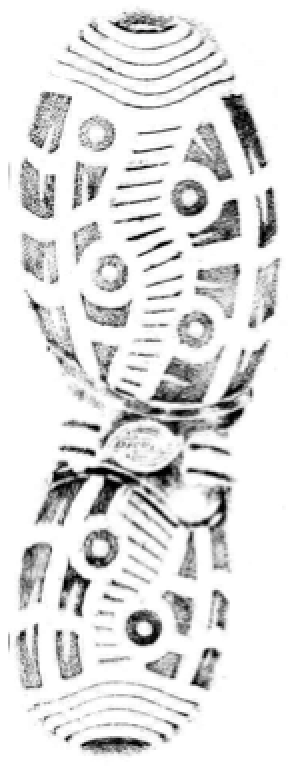
\includegraphics [width=0.1\linewidth]{Figures/FootwearK}
}
\subfigure[Features]{
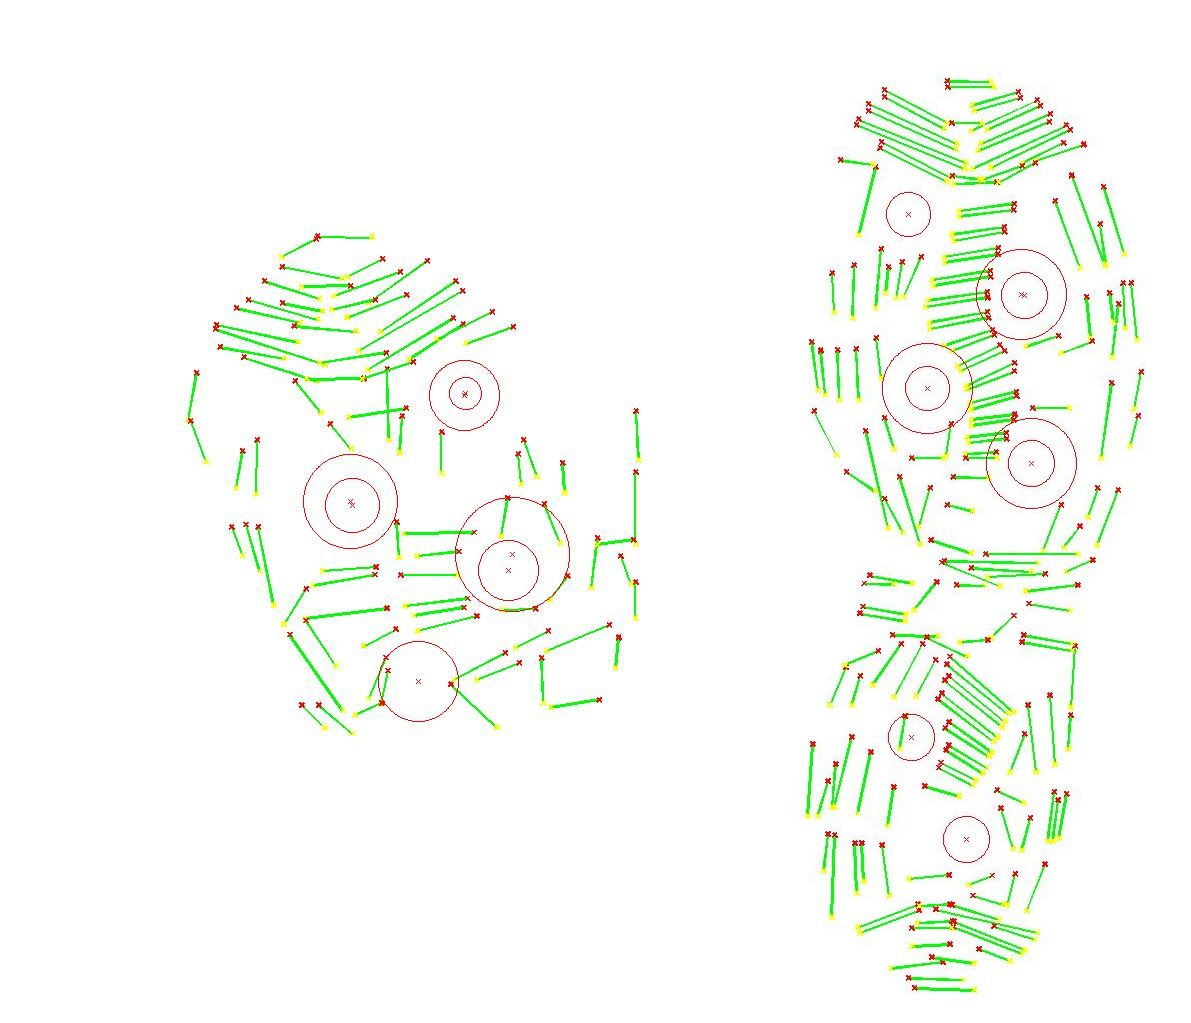
\includegraphics [width= 0.35\linewidth]{Figures/shoe_houghresults}
}
\subfigure[Nodes in graphs]{
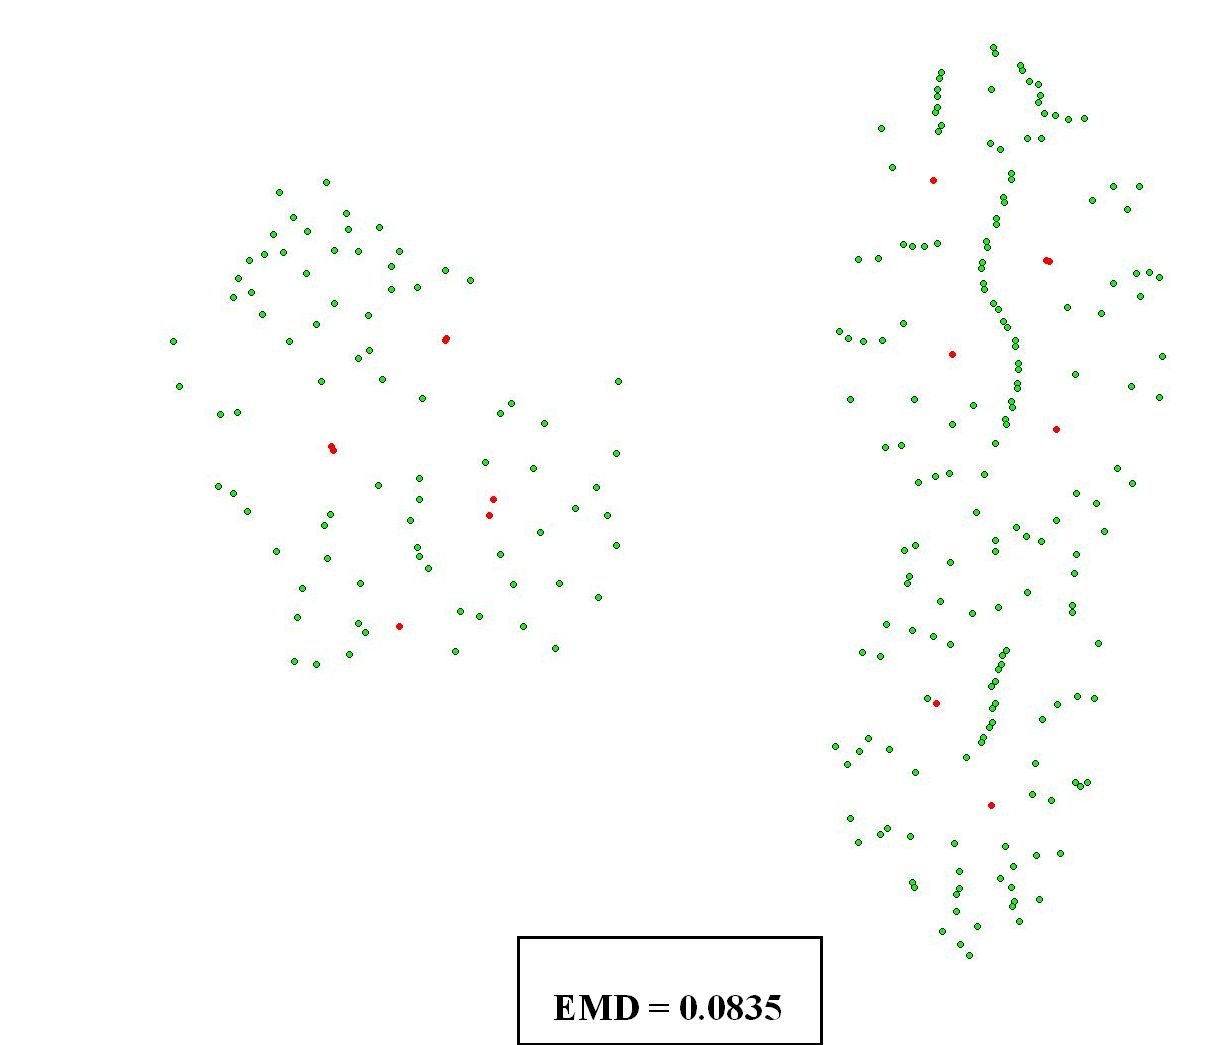
\includegraphics [width=0.35\linewidth]{Figures/shoe_graphs}
}
\caption{\small{Footwear impression evidence analysis: (a) crime scene print,  (b)  its known source, (c) detected features (centers of circles) in evidence and known, and (d)  graph representations of evidence and known (edges not shown).   A modified earthmover distance (EMD) between graphs is used to determine $LR_D$ (from \cite{Srihari2011a,Srihari2014}).}}
%\end{minipage}
\label{fig:Footwear}
\end{figure}




\section{PROPOSED RESEARCH AND CAPACITY BUILDING} 
\label{Section:proposed}
The proposed work will  investigate different deep neural network architectures  for forensic comparison, performing  experiments with data sets from two forensic impression evidence domains.
%\subsection{Discriminative Models}
We begin by noting that (\ref{eq:LRJ}) can be rewritten as
\begin{equation}
LR(\phi_{k},\phi_{e})=\frac{p[({\bf \phi}_k,{\bf \phi}_e) | h^{0}]}{p[({\bf \phi}_k ,{\bf \phi}_e) | h^{1}]}
=\frac{p[h^{0}|\phi_k , \phi_e]p(h^{1})}{p[h^{1}|\phi_k , \phi_e]p(h^{0})}
=\frac{p(h^{0}|\phi_e , \phi_k )}{1-p(h^0 | \phi_e , \phi_k )}
\label{eq:discriminative}
\end{equation}
where we have assumed equal priors, $p(h^0 )=p(h^1)$.   LR  can be directly determined using a neural network with a single hidden layer  as follows:
\begin{equation}
p(h^{0}|\phi )=\sigma_{1} \left( \sum_{j=1}^{M} w_{j}^{(2)}\sigma_{2} \left (\sum_{i=1}^{D} w_{ji}^{(1)}\phi_{i}+b_{1} \right) + b_{2} \right)
\label{eq:neuralnet}
\end{equation}
where $\phi=(\phi_{e},\phi_{k})$ has $D$ components;   $w_{j}^{(2)}, w_{ji}^{(1)}, b_{1},b_{2}$ are parameters determined from supervised training data; $\sigma_{1}$ is an activation function (either sigmoid or probit); $\sigma_{2}$ is another activation, possibly  ReLU; and $M$ is model complexity (no. of hidden units).
A toy example of both models (generative and discriminative)  is shown in Fig. \ref{fig:GenDisc}, where the computed  LRs are quite close.  Our research will explore architectures  with multiple layers, different levels of model complexity. 

The task differs from classic object recognition, e.g., handwritten digit recognition,  in that we have two inputs rather than one. Interlacing the two inputs $\phi_{e},\phi_{k}$ is a significant issue, since the goal is to learn minor differences between objects that are otherwise quite similar.  Forensic comparison thus focuses on individuality while ignoring average over the population, i.e, we are interested in the tails of the distribution (of shape).   Conversely, object recognition concerns how similar the object is to the mean/mode of the distribution.


\begin{figure}
\centering
\tiny
\subtable[Parameters of generative model.]{
\begin{tabular}{ccc}
\hline 
$\phi_{e},\phi_{k}$ & $p\left(\phi_{e},\phi_{k}|h^{0}\right)$ & $p\left(\phi_{e},\phi_{k}|h^{1}\right)$\tabularnewline
\hline 
00,00 & 0.1957 & 0.0296\tabularnewline
00,01 & 0.0217 & 0.0740\tabularnewline
00,10 & 0.0326 & 0.0592\tabularnewline
00,11 & 0.0022 & 0.1405 \tabularnewline
01,00 & 0.0217  & 0.0592\tabularnewline
01,01 & 0.1739 & 0.0148\tabularnewline
01,10 & 0.0043 & 0.0740\tabularnewline
01,11 & 0.0217 & 0.0740\tabularnewline
10,00 & 0.0283 & 0.0888\tabularnewline
10,01 & 0.0152 & 0.1036\tabularnewline
10,10 & 0.1935 & 0.0296\tabularnewline
10,11 & 0.0435 & 0.0592\tabularnewline
11,00 & 0.0022  & 0.0015\tabularnewline
11,01 & 0.0217 & 0.0888\tabularnewline
11,10 & 0.0217 & 0.0888\tabularnewline
11,11 & 0.2000 & 0.0148 \tabularnewline
\hline 
\end{tabular}
%\protect
%\par\end{centering}
}
\subfigure[A discriminative model: neural network for computing $p(h^{0}|\phi_{k}.\phi_{e})$ . It was trained using learning-rate = 0.01, mini-batch-size = 100, and no. of iterations = 300.
The number of generated samples was 20,000.]{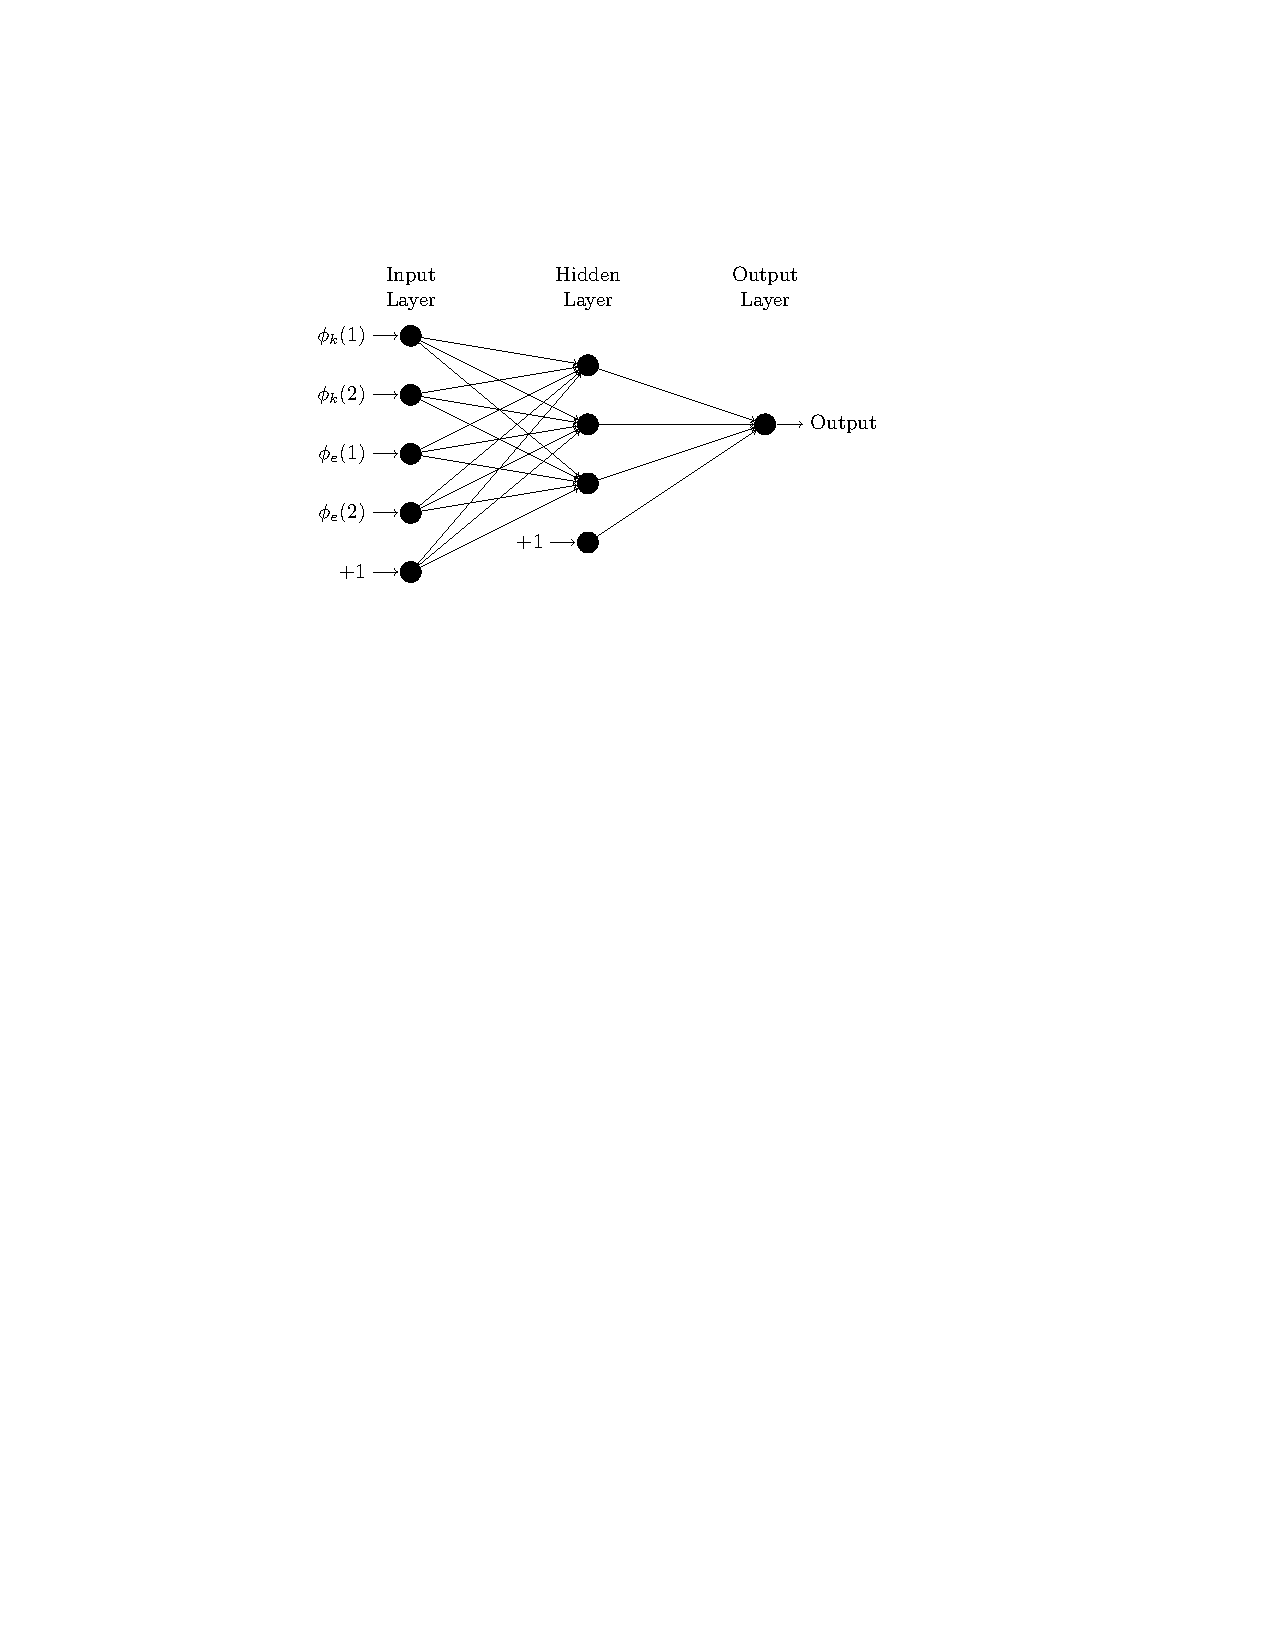
\includegraphics[width=0.5\linewidth]{Figures/nn431}}
\subtable[Parameters of neural network (weights and biases)]{
%\begin{center}
\begin{tabular}{ccccc}
w11&-5.5169 & 2.7104 & 5.8524 & -0.7585\tabularnewline
w12&-5.4884 & -4.807 & 4.6924 & 6.5\tabularnewline
w13&0.6106 & -5.8483 & -3.2345 & 5.8516\tabularnewline
b1&-3.9789&0.5988&-1.6443&\tabularnewline
w2&5.9490 & -4.3345 & 5.8192\tabularnewline
b2&0.2064&&&\tabularnewline
%w11&-3.0969 & -2.7141 & 0.1235 & 0.239\tabularnewline
%w12&-4.9126 & -10.4361 & 3.9566 & -2.9961\tabularnewline
%w13&-9.4213 & -2.2776 & -6.0361 & 1.6116\tabularnewline
%w2&19.7844 & -10.4502 & -12.3178\tabularnewline
\end{tabular}
}
\subtable[Values of hidden layer activations]{
\begin{tabular}{cccc}
\hline 
Input & Hidden Node 1 & Hidden Node 2 & Hidden Node 3\tabularnewline
\hline 
 0 0 0 0 & 0.0184 & 0.6454 & 0.1619\tabularnewline
 0 0 0 1 & 0.0087 & 0.9992 & 0.9853\tabularnewline
 0 0 1 0 & 0.8669 & 0.995 & 0.0075\tabularnewline
 0 0 1 1 & 0.7531 & 1 & 0.7257\tabularnewline
 0 1 0 0 & 0.2195 & 0.0147 & 0.0006\tabularnewline
 0 1 0 1 & 0.1164 & 0.9082 & 0.1623\tabularnewline
 0 1 1 0 & 0.9899 & 0.6187 & 0\tabularnewline
 0 1 1 1 & 0.9787 & 0.9991 & 0.0076\tabularnewline
 1 0 0 0 & 0.0001 & 0.0075 & 0.2624\tabularnewline
 1 0 0 1 & 0 & 0.8335 & 0.992\tabularnewline
 1 0 1 0 & 0.0255 & 0.4509 & 0.0138\tabularnewline
 1 0 1 1 & 0.0121 & 0.9982 & 0.8297\tabularnewline
 1 1 0 0 & 0.0011 & 0.0001 & 0.001\tabularnewline
 1 1 0 1 & 0.0005 & 0.0393 & 0.263\tabularnewline
 1 1 1 0 & 0.2823 & 0.0067 & 0\tabularnewline
 1 1 1 1 & 0.1556 & 0.817 & 0.0139\tabularnewline
\hline 
\end{tabular}
}
\subfigure[Likelihood ratios using the generative model (red) and the discriminative model (blue). The two models show similar values, with peaks corresponding to $\phi_{k}=\phi_{e}$.]{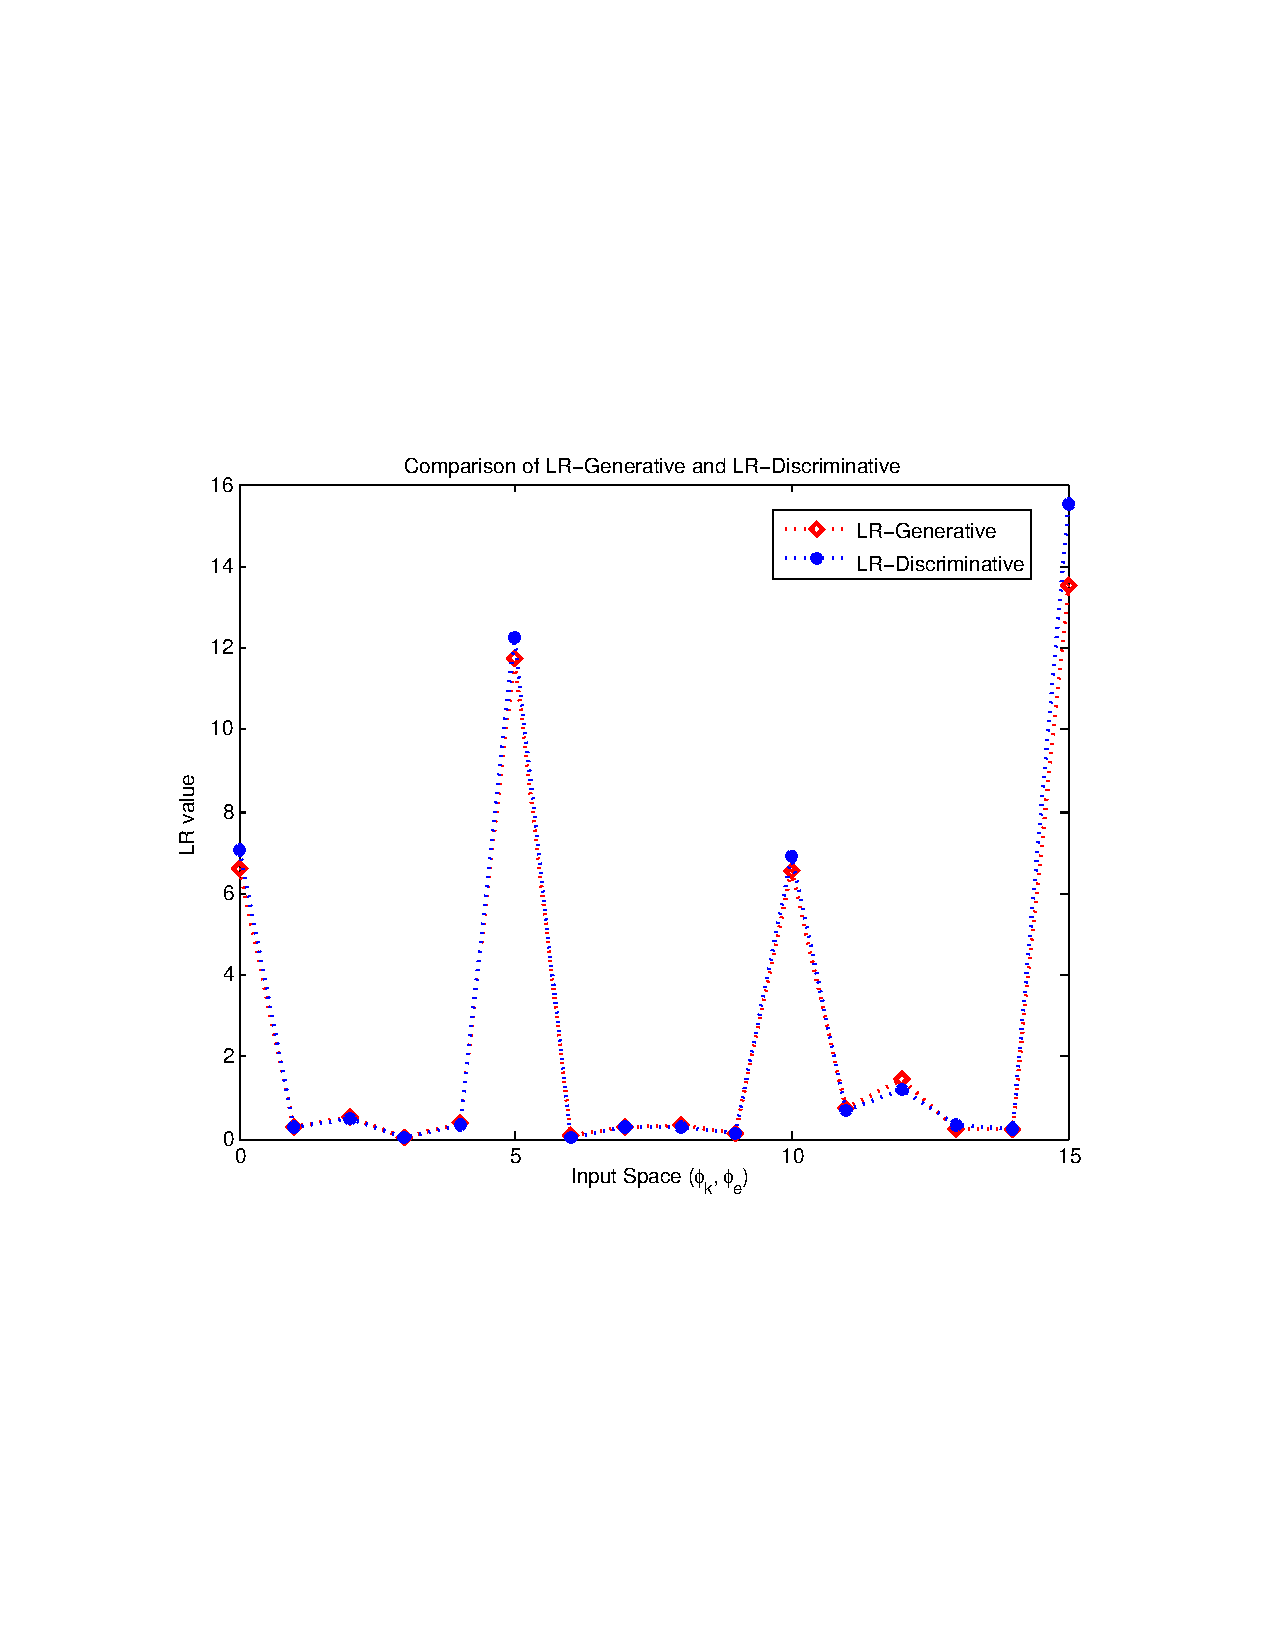
\includegraphics [width=0.5\linewidth]{Figures/nnLR}}
\caption{Two models for determining $LR(\phi_{k}.\phi_{e})$: (a) generative model (16 probabilities) when $\phi_k$ and $\phi_e$ are represented by two bits each, (b) discriminative model: neural network with 4-3-1 nodes with output $p(h^{0}|\phi )=\sigma\left[W_{2} {\bf \sigma}\left(W_{1} \phi +b_{1}\right)+b_{2}\right]$, (c) weights and biases of the neural network, (d) activation values, and  (e) $LR(\phi_{k},\phi_{e})$ for the sixteen possible inputs using both models;  peak values occur when $\phi_{k}=\phi_{e}$ (reflecting exact match), and extremely low values occur when $\phi_{k}=\overline{\phi_{e}}$ (exclusion). }
\label{fig:GenDisc}
\end{figure}



\subsection {Deep Learning Architectures}

We propose to evaluate several architectures for the forensic comparison task. We will begin with human extracted features for handwriting (as seen in Fig. \ref{fig:th-features}) and automatically extracted features for footwear impressions (as seen in Fig. \ref{fig:Footwear}) and then proceed to  raw images as input. As we have seen earlier,  even when we have human extracted features,  the generative approach is infeasible due to  exponential complexity.  Thus a discriminative solution based on such features itself would be of great benefit to the forensic community. If we eventually succeed with raw images, we would circumvent the need for human and machine-effort in feature extraction.

For these experiments we will explore both conventional neural network and   convolutional  neural network (CNN) architectures.  One design  consists of separate networks for inputs $\phi_{k}$  and $\phi_{e}$ with shared weights, with the results combined at later stages, as shown  in Fig. \ref{fig:cnn}.  Another design would interlace the two inputs so that minor feature differences can be learnt-- while such as design comes closer to our earlier design (Fig. \ref{fig:NN-JFS}),  it does not lose information through a distance/kernel function.

First, we will try and see how handwriting comparison performs
with  a single-hidden-layer densely connected neural
network. Then we add a convolution layer together with a pooling
layer on top of the input layer and see how  performance changes.
If  performance improves, we can try adding another convolution
layer and a pooling layer. Each time we add a new convolution-pooling
layer the number of feature maps increases by a certain factor. The
final output of all convolution-pooling layers will go into a final
densely connected layer. At first, the number of nodes in the densely
connected layer is small, so that the model does not overfit the training
data in the last layer. Then we gradually increase the number of nodes
in the final densely connected layer until  performance stops increasing.


Nonlinear activation functions suitable for LR computation will be explored. The ReLU\footnote{Rectifier Linear Unit has become most popular for deep learning.} has become popular for earlier stages. A  probit for the final output  may be useful to avoid extremely large/small LRs. 
A probit function provides a gradual transition between the two output states (Fig. \ref{fig:Probit}). Since probit is a cdf of a Gaussian, its variance can be determined from training data. 
 \begin{figure}
 \centering
 \includegraphics[width=0.3\linewidth]{Figures/Probit.pdf}
 \caption{Probit non-linear activation function. It is the cdf of a Gaussian, whose standard deviation is determined from training data}
  \label{fig:Probit}
 \end{figure}



\begin{figure}
\centering
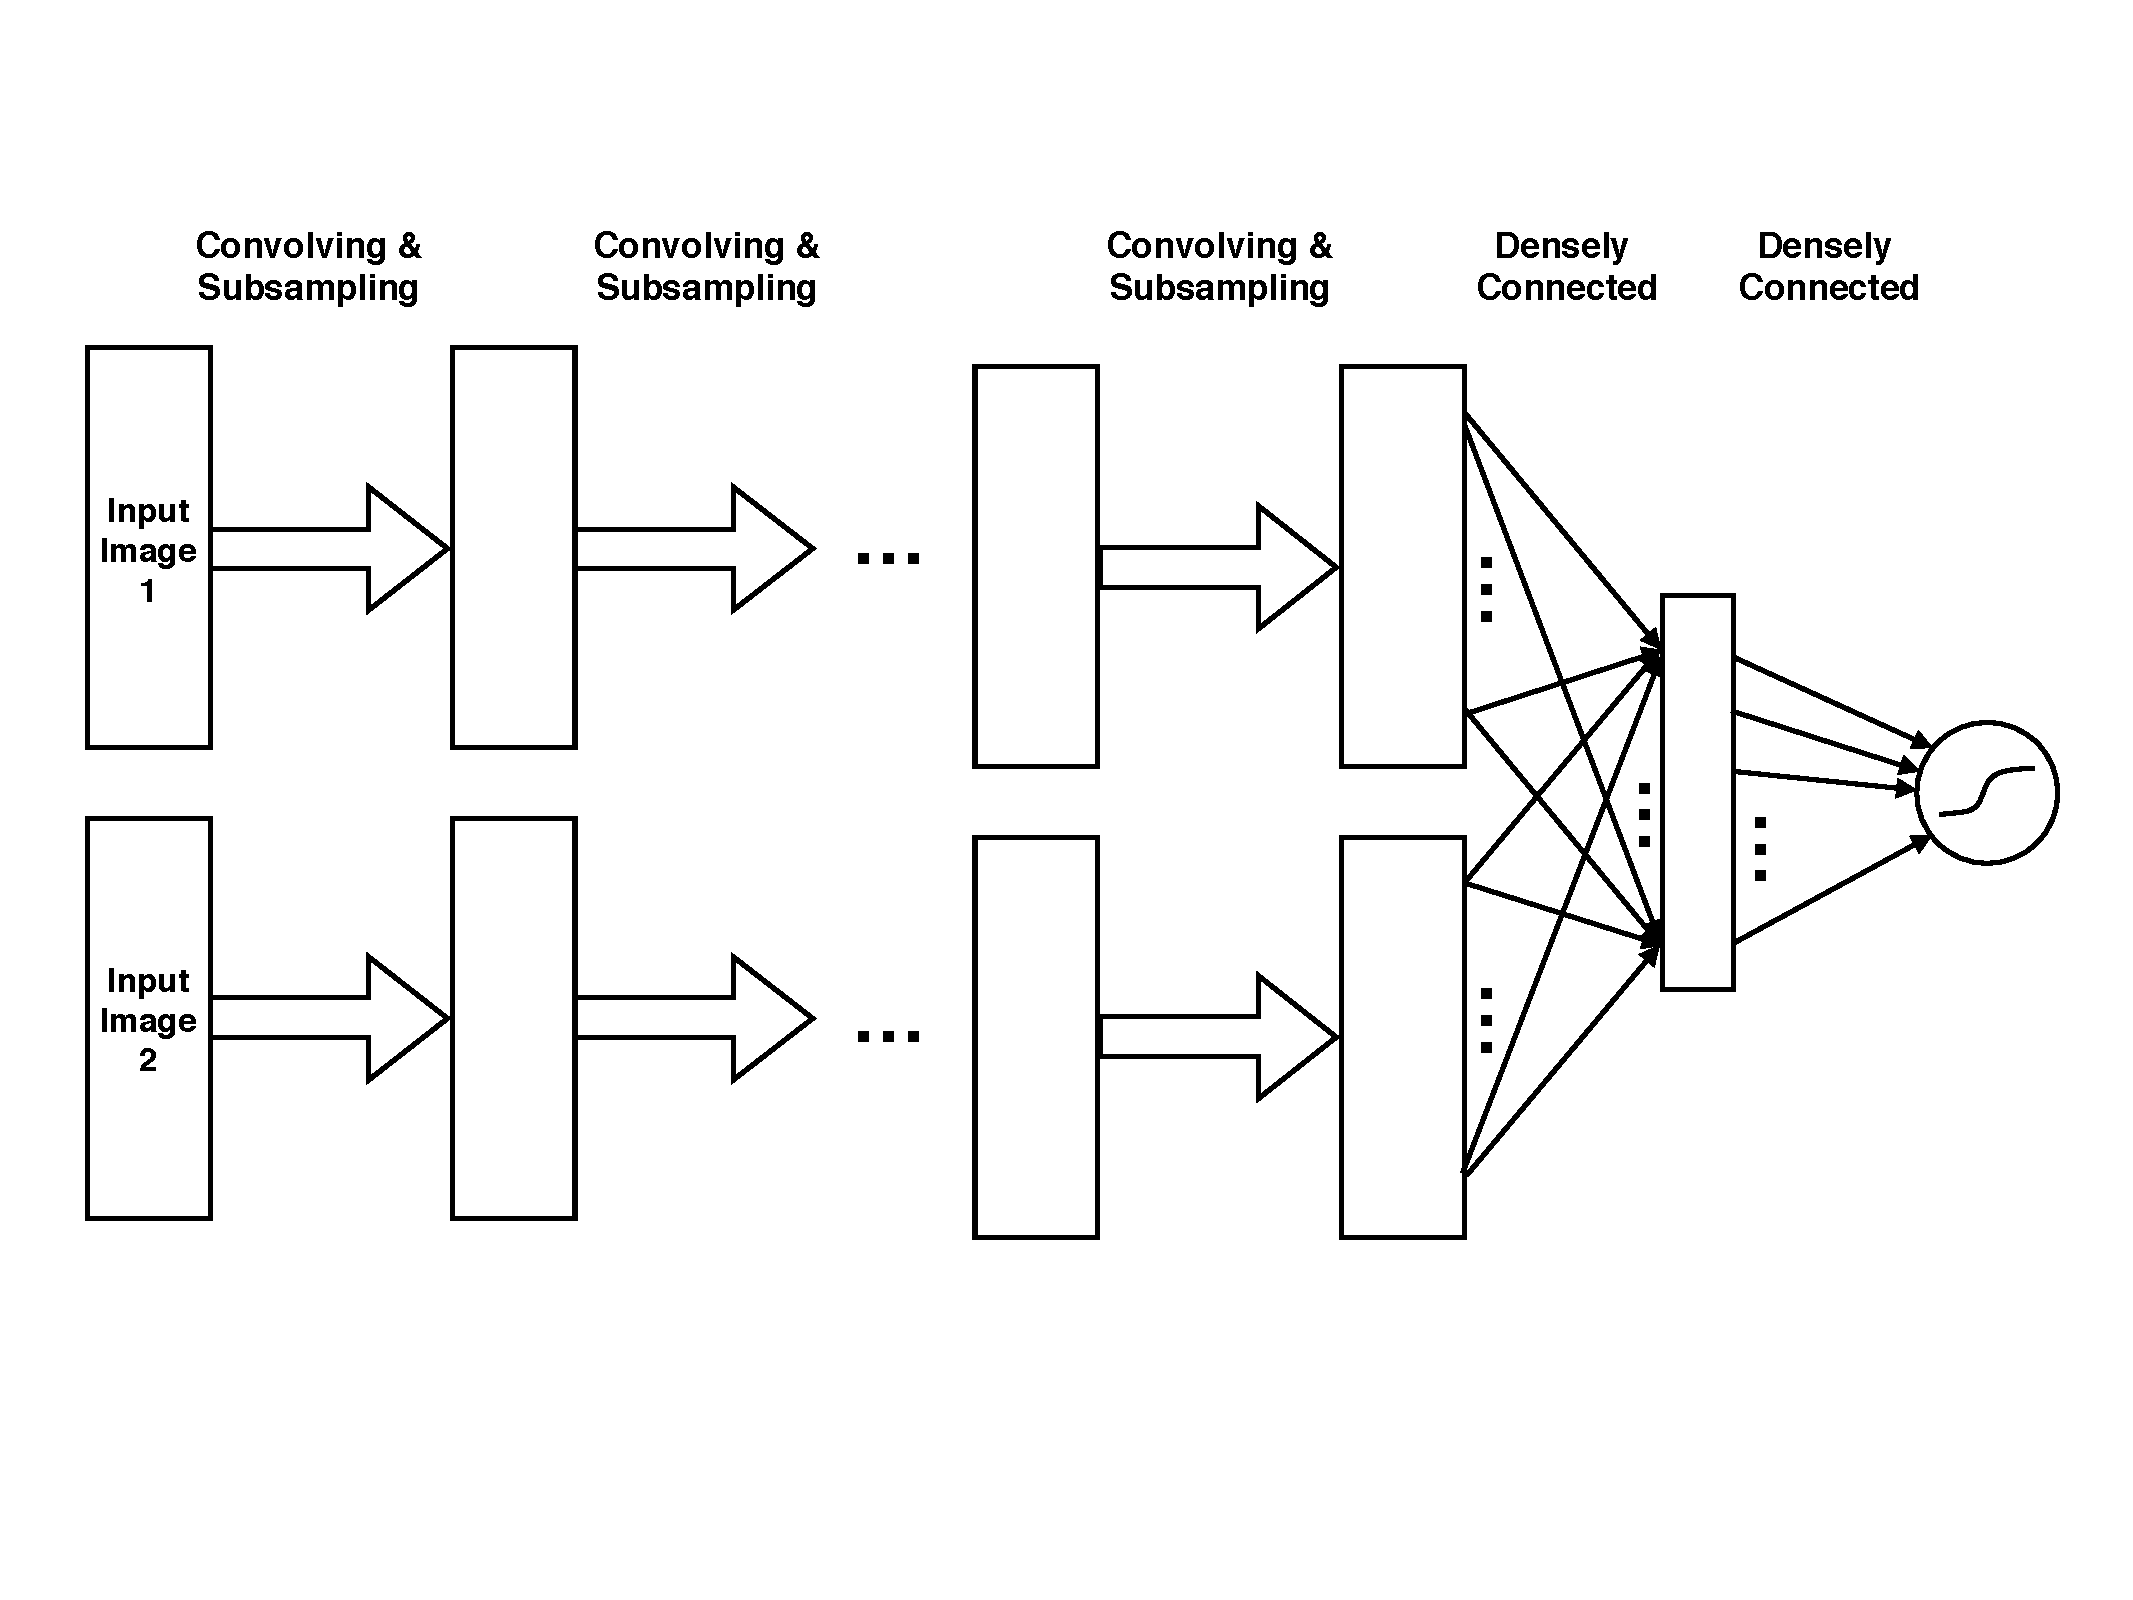
\includegraphics[width=0.6\textwidth]{Figures/cnn}
\caption{A proposed convolutional neural network  for  LR computation.}
\label{fig:cnn}
\end{figure}




 \subsection{Learning Algorithms}
 
The principal method to update weights  in deep learning is SGD with the key equation
$
{\boldmath {\mathrm w}}^{\tau +1}={\boldmath {\mathrm w}}^{\tau }-\eta \nabla E, 
$
where $\nabla E$, partial derivatives with respect to the weights,  is determined in mini-batches using error back propagation and $\eta$ is the learning rate. Local minima are not a serious problem for deep learning since several minima provide similar results \cite{LeCun2015}. While SGD is efficient, further speed-up is possible with  line search and conjugate descent. Contrastive divergence is useful  if we  incorporate into the network a generative model, such as a Restricted Boltzmann Machine (RBM), to determine features. 

Training will require several experimental settings, e.g., no. of convolutional layers, no. of nodes in each layer, no. of feature maps, size of  filters, size of  pooling size, kind of regularization,  learning rate, etc.
As an example, for learning rate we first choose a small portion of the training data and pick up an initial try  and iterate SGD for a few loops. If the
loss function is observably decreasing, then we can double the learning
rate in the next try. If the loss does not go down in the first few
iterations, then perhaps we picked up too big a learning rate and
SGD will not converge. The next try will use half of the original value. This process is continued until we
find a  learning rate that converges fast.

\subsection{Regularization}
Our preliminary  experiments show that simple models tend to overfit, e.g., although the  error on the training data is small,  error on testing is hard to enhance. 
Data augmentation is one method of regularization that other researchers have found to be effective.  We introduce some distortion or perturbation to produce new data, an example of which is given in Fig. \ref{fig:augmentation}. 

\begin{figure}
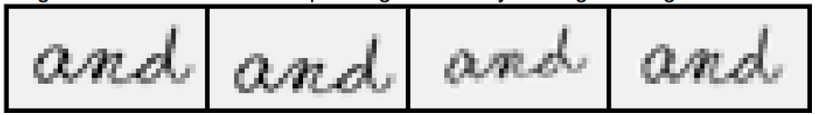
\includegraphics[width=0.5\linewidth]{Figures/AugmentedData}
\caption{Data augmentation using transformations: translation, rotation, scaling and squeezing.}
\label{fig:augmentation}
\end{figure}

Standard methods of regularization used in machine learning, e.g., those based on minimizing the Lagrangian with $L_{2}$ , $L_{1}$ can also be used. More recently regularization of  large fully-connected   neural networks by setting a randomly selected subset of activations in each layer to zero, called dropout \cite{Srivastava2014} ,  and drop-connect \cite{Wan2013} (where a randomly  selected subset of weights are set to zero) have been proposed.  We will experiment with each of these or a combination of them. They are all controlled by a coefficient, which can be determined by observing model performance on a separate validation set.

\subsection{Multiple Evidence Combination}
We will explore three evidence combination approaches:
The first assumes  independent comparisons.
For  $K$ comparisons, with features  $\Phi_{k}=\{ \phi_{k_i} \}^{K}_{i=1}$ and $\Phi_{e}=\{ \phi_{e_i} \}^{K}_{i=1}$, we get:
\begin{equation}
\label{eq:EqMain}
p(h^{0}|\Phi_{k} , \Phi_{e}) = \dfrac{p(h^{0})\cdot \prod_{i=1}^{K}LR(\phi_{k_i}, \phi_{e_i})}{p(h^{1}) + p(h^{0})\cdot \prod_{i=1}^{K} LR(\phi_{k_i},\phi_{e_i})}
\end{equation}
where:
$LR(\phi_{k_i},\phi_{e_i}) = \frac{p(\phi_{k_i},\phi_{e_i}|h^{0})}{p(\phi_{k_i},\phi_{e_i}|h^{1})}$. The posterior probability in  (\ref{eq:EqMain}),  can be converted into  $LR(\Phi_{k},\Phi_{e})$ by using (\ref{eq:discriminative}).
Since  this result is not always satisfactory, e.g., we can get nearly the same value $LR(\Phi_{k}, \Phi_{e})$ based on many comparisons or only a few  comparisons, alternative weighting methods can be used \cite{Kovalenko2012}. In the second approach  dependencies between comparisons use either generative HMMs or discriminative CRFs \cite{Koller2009}, where each observation and latent node of the PGM would have two variables. The third method  is Recurrent Neural Networks (RNN) which have done well in natural language processing\cite{LeCun2015}.


\subsection{Data Sets for Training Models}
We will use data from two different impression evidence modalities:
\begin{enumerate}
\item {\em Handwriting}: we have several handwriting data sets available for this research:
\begin{enumerate}
\item Scanned full page writings of 1,500 adults representative of the US population:  3 pages per writer ( allows same/different comparisons)  \cite{Srihari2002}. Snippets shown in Fig. \ref{fig:US-examples}.
\item Paragraphs of handwriting of children in grades 2-4 over a period of three years. Which allows study of growth of handwriting individuality as they grow older \cite{SrihariHanson2014}.
\item Extracted  and truthed {\em th} and {\em and} images together with FDE-assigned feature values (twelve features for {\em and} are shown in Fig. \ref{fig:and-features}). They were chosen because {\em th}, {\em an} and {\em nd} are among the the most common bigrams in the English language. There are 888 writing samples from children over three years.
\end{enumerate}

\begin{figure}[t!]
\centering
%\subfigure[]{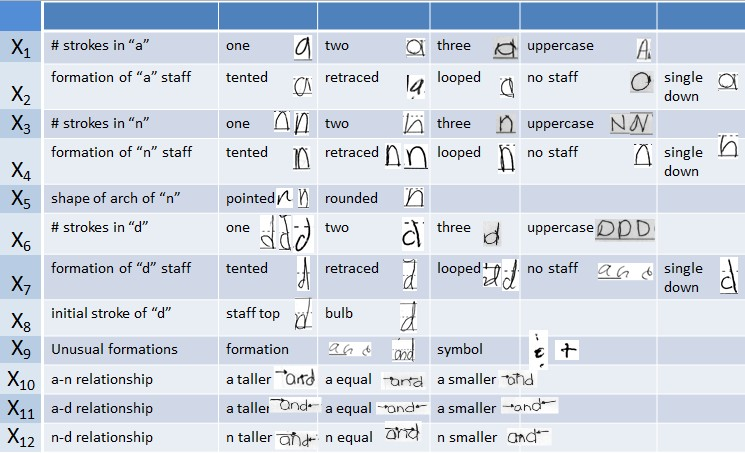
\includegraphics[width=0.475\linewidth]{figures/and_features_printed}}
\subfigure[]{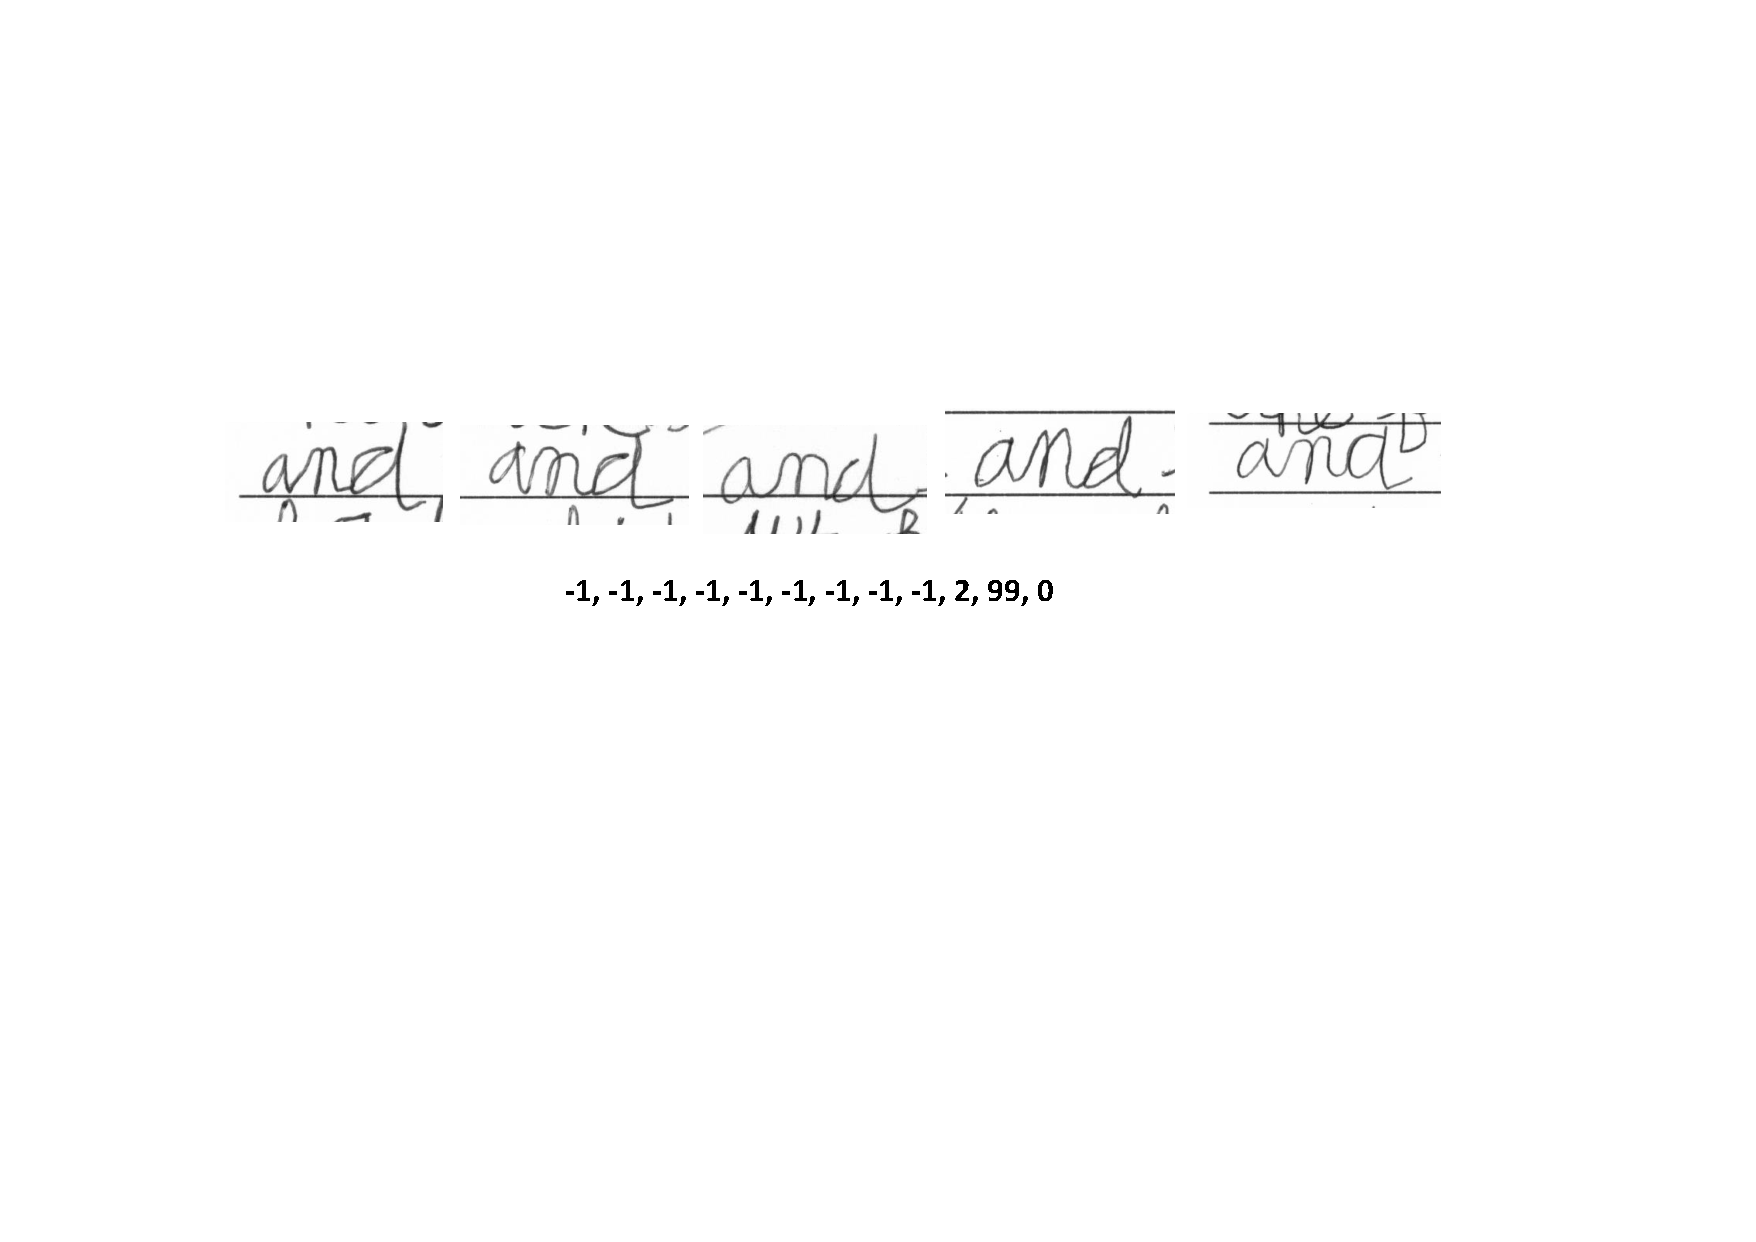
\includegraphics[width=0.48\linewidth]{figures/Missing_cursive}}
\subfigure[]{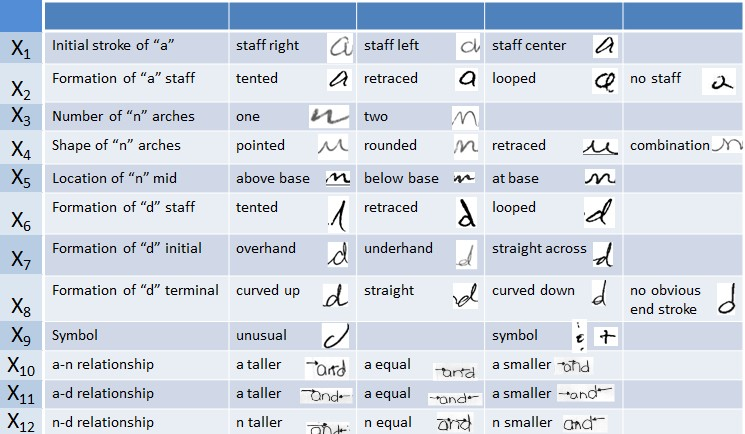
\includegraphics[width=0.48\linewidth]{figures/and_feature_cursive}}
\caption{ Handwritten {\em and} data.: (a) images for a single writer, and  (b) features definition table.  }
\label{fig:and-features}
\end{figure}

%\begin{figure}[t!]
%\centering
%\subfigure[]{\includegraphics[width=0.485\linewidth]{figures/Missing_printed_1}}
%\subfigure[]{\includegraphics[width=0.485\linewidth]{figures/Missing_cursive_1}}
%\caption{ Examples of two sets of images corresponding to two feature values, which contain incommensurate ($99$) and missing ($-1$) values. (a) Printed \emph{and}. (b) Cursive \emph{and}.}
%\label{fig:miss_example}
%\end{figure}
%


\item {\em Footwear prints}: Several hundred crime scene and standard footwear prints are available \cite{Srihari2011a}.  Some examples are shown in Fig.  \ref{fig:Footwear}.
\end{enumerate}
Since much of the success of deep learning has come from the availability of huge data sets, we will address it as follows:
\begin{enumerate}
\item Augment image data sets by subjecting the given samples to various transformations, e.g., translation, rotation, scaling, deformation.
\item Extract some preliminary features, e.g., for footwear images using methods described in \cite{Srihari2011a},  and perform discriminative training above that level.
\end{enumerate}

 \subsection{GPU implementation}
 Since CNN training usually involves intensive computation, a GPU for the training task is indispensable. Compared to a CPU, a GPU has a
huge amount of computing unit that can perform parallel computation which is very advantageous for matrix operations like convolution.
There are various implementations of the GPU library for matrix operations. For our implementation, we could use Theano
\footnote{Theano is a utility package for Python  to realize CNN models. We first write code to construct mathematical relationships between symbolic variables, e.g., relations between input, weights, output, loss functions. We can also specify parameters for SGD (epochs, mini-batch size, eta, lambda, etc).  Theano will compile C code for such functions to achieve better run-time performance. After that, we can simply use them as a normal Python function and feed in data to compute results.}, 
which is a Python library that supports GPU computation. One advantage is that it can perform automatic differentiation.
The NVIDIA Tesla K40 graphic card is available for {\$}3,000 which we propose to acquire for this research.



\section{Project Milestones and Timeline}
\label{Timeline}
 
\begin{enumerate}
\item{September 1, 2016: 	Begin studies on neural networks for forensic comparison.}
\item{December 31, 2016:  Complete  preparing evidence-known data sets using data augmentation.}
\item{August 31, 2017:  Complete study of neural network methods for (i) human extracted features for handwriting and (ii) machine-extracted features for footwear impressions.}
\item{August 31, 2018: Complete Deep Learning implementations for raw images of handwriting and footwear impressions.}
\item{June 31  2019:  Refine Deep Learning Methods and Complete Evidence Combination studies.}
\item{August 31, 2019: Write-up final conclusions and prepare report}
\end{enumerate}



\section{Capacity Building: Curriculum Development Activities}

The PI teaches courses on ML and PGMs. The ML course has seniors and first year undergraduates (135 students for ML  and 60  for PGM in 2015). The material is  updated each year and the lectures with presentations  are made freely available at \url{http://www.cedar.buffalo.edu/~srihari/CSE574}.  Students are assigned several programming projects.  
Projects related to this research will provide students  exposure to forensic  problems as well as deep learning. 


\section{Intellectual Merit}
Three new concepts are to be explored: (i)  a  discriminative model  to arrive at a probabilistic statement in forensic comparison,  (ii) deep neural networks to work with two inputs rather than one (evidence and known), and (iii) obtaining a single probabilistic opinion using several comparisons. 

\section{Broader Impacts of the Proposed Work}
The forensic sciences are at a crisis mode at present-- since many currently used methods, based on human expertise, largely do not satisfy legal requirements of having a scientific basis. The probabilistic method proposed in this research has the potential of providing a dramatic break-through, not only to the forensic domains used in this research but also to other forensic domains as well, e.g., latent prints, video evidence, etc.
\section{Results from Prior NSF Support}
 {\bf Project ID and Title}: IIS-0750876, 2007-09,  {\em Recognition of Handwritten Words in School Essays Using Conditional Random Fields}, \$100,000.  
\subsection{Intellectual Merit} 
Contextual dependency between words was use in recognition using CRFs. Resulting method was made part of a system to score handwritten essays.
Published  in:
S. N. Srihari, J. Collins, R. K. Srihari, H. Srinivasan, S. Shetty, and J. Brutt-Griffler, ``Automatic Scoring of Short Handwritten Essays in Reading Comprehension Tests," Artificial Intelligence, vol. 172(2-3) 2008, pp. 300-324.
\subsection{Broader Impacts}
First paper to describe how schools can automate scoring of handwritten essays. Success in the task would lead to  students receiving performance results earlier in the school year which would enhance their learning.

\newpage
\pagenumbering{roman}
\bibliographystyle{IEEEtran}
\bibliography{ProjectDescription}

\end{document}